\documentclass[journal=esthag,manuscript=article]{achemso}

% additional packages
\usepackage[utf8]{inputenc}
\usepackage{amsmath}
\usepackage{booktabs}
\usepackage{subcaption}
\usepackage{tabularx}
\usepackage{array,multirow,graphicx}
\usepackage{comment}
\graphicspath{
  {./../figures/},
  {./../figures/air-exchange-rate/},
  {./../figures/kde-iacc-pressure/},
  {./../figures/preferential-pathway-sensitivity/},
  {./../figures/transient-response/},
  {./../figures/multivariate_analysis/},
  {./../figures/rate_of_change/},
}
\usepackage{lineno}
\linenumbers
% macros

% authors
\author{Jonathan G. V. Ström}
\affiliation[Brown University]{Brown University, School of Engineering, Providence, RI, USA}
\author{Yijun Yao}
\affiliation[Zhejiang University]{Zhejiang University, Hangzhou, China}
\author{Eric M. Suuberg}
\email{eric_suuberg@brown.edu}
\affiliation[Brown University]{Brown University, School of Engineering, Providence, RI, USA}

% title
\title{Transient Variability In Vapor Intrusion And The Factors That Influence It}

% keywords
\abbreviations{VI}
\keywords{VI, Preferential pathways, Temporal transient variability}

\begin{document}

\begin{abstract}
Temporal variability in indoor air contaminant concentrations at vapor intrusion (VI) sites has been a concern for some time.
We consider the source of the variability at VI sites located near Hill Air Force Base in Utah, an EPA experimental house in Indianapolis, IN and Naval Air Station North Island in California using statistical analysis methods and three-dimensional subsurface computational fluid dynamics modeling.
The results suggest that an order of magnitude variation in indoor air contaminant concentrations may be expected at ”normal” VI sites where preferential pathways do not play a role, whereas three or more orders of magnitude can be observed at sites characterized by preferential pathways.
A computational fluid dynamics modeling sensitivity analysis reveals that it is not only the presence of contaminant vapor in a preferential pathway that is required to see large observed variations, but there must also exist a permeable region beneath the structure.
Large temporal fluctuations in indoor air contaminant concentrations may be observed where no preferential pathways exist, but this requires a particular combination of large fluctuations in pressure driving force and high soil permeability.
\end{abstract}

\section{Introduction}

Long term vapor intrusion (VI) studies in both residential and larger commercial structures have raised concerns regarding significant observed transient behavior in indoor air contaminant concentrations\cite{u.s._environmental_protection_agency_oswer_2015,folkes_observed_2009,holton_temporal_2013,johnston_spatiotemporal_2014,hosangadi_high-frequency_2017,mchugh_recent_2017,u.s._environmental_protection_agency_assessment_2015}.
VI involves the migration of volatilizing contaminants from soil, groundwater or other subsurface sources into overlying structures. VI has been a recognized problem for some time, but many aspects remain poorly understood, particularly with respect to the causes of large temporal transients in indoor air concentrations.
There is uncertainty within the VI community regarding how to best develop sampling strategies to address this problem\cite{u.s._environmental_protection_agency_oswer_2015,holton_temporal_2013,johnson_integrated_2016}. \par

Results from a house operated by Arizona State University (ASU) near Hill AFB in Utah, an EPA experimental house in Indianapolis, IN and a large warehouse at the Naval Air Station (NAS) North Island, CA have all shown significant transient variations in indoor air contaminant concentrations.
All were outfitted with sampling and monitoring equipment that allowed tracking temporal variation in indoor air contaminant concentrations on time scales of hours.
All have shown that these concentrations varied significantly with time - orders of magnitude on the timescale of a day or days.
\cite{holton_evaluation_2015,guo_vapor_2015,hosangadi_high-frequency_2017}. \par

In one instance the source of the variation was clearly established during the study; at the ASU house a field drain pipe (or “land drain”), which connected to a sewer system, was discovered beneath the house, and careful isolation of this source led to a clear conclusion that this preferential pathway significantly contributed to observed indoor air contaminant levels and their fluctuations\cite{guo_vapor_2015,guo_identification_2015}.
While in this case the issue of a contribution from a preferential pathway was clearly resolved, what it left open was a question of whether existence of such a preferential pathway to an area beneath a structure would always be expected to lead to large fluctuations in indoor air contaminant concentrations. \par

Similarly, a sewer pipe has recently been suggested to be a source of the contaminants found in the EPA Indianapolis house.
That site was also characterized by large indoor air contaminant concentration fluctuations\cite{mchugh_evidence_2017,u.s._environmental_protection_agency_assessment_2015}.
Sewer lines have been generally implicated as VI sources at several sites\cite{pennell_sewer_2013,mchugh_evidence_2017,roghani_occurrence_2018,riis_vapor_2010}.
A Danish study estimate that roughly 20\% of all VI sites in central Denmark involve significant sewer VI pathways\cite{nielsen_remediation_2017}.
Thus while the consideration of a role of possible sewer or other preferential pathways is now part of normal good practice in VI site investigation\cite{u.s._environmental_protection_agency_oswer_2015}, it is still not known whether the existence of such pathways automatically means that large temporal fluctuations are necessarily to be expected.
In some of these cited cases\cite{pennell_sewer_2013,riis_vapor_2010}, a sewer provided a pathway for direct entry of contaminant into the living space.
While potentially important in many cases, this scenario is not further considered here, where the focus is on pathways that deliver contaminant via the soil beneath a structure. \par

It is, however, now known that even absent a preferential pathway, there may be significant transient variation in indoor air contaminant concentrations at VI sites\cite{folkes_observed_2009,brenner_results_2010,johnston_spatiotemporal_2014}.
One example is a site at NAS North Island at which no preferential pathways have been identified.
Instead, a building at this site is characterized by significant temporal variations in indoor-outdoor pressure differential\cite{hosangadi_high-frequency_2017}.
It is believed that this is the origin of the observed indoor air contaminant concentration fluctuations at that site. \par

This paper investigates the sources of the temporal variation in indoor air contaminant concentrations in both the presence and absence of preferential pathways.
In this work, the latter scenarios are referred to as ”normal” VI scenarios, in which there is typically a groundwater source of the contaminant.
Specifically, we pose the question of just how much variation in indoor air contaminant concentration may be expected at  such normal  VI  sites vs. those characterized by preferential pathways.
The conditions required for preferential pathways to become significant contributors to temporal variations in indoor air contaminant concentrations are also explored, and the consequences for sampling strategies are also discussed.

\section{Methods}

\subsection{Statistical Analysis Of Field Data}

To begin to characterize transient behavior in indoor air contaminant concentrations, actual datasets are analyzed to establish common levels of variability at VI sites.
For this purpose, the datasets from the ASU house in Utah, the EPA Indianapolis site and North Island NAS were chosen for analysis.
This paper relies on statistical analysis of published field data, and readers are referred to the original works for details regarding data acquisition\cite{holton_evaluation_2015,guo_vapor_2015,holton_temporal_2013,hosangadi_high-frequency_2017,u.s._environmental_protection_agency_assessment_2015}. \par

The ASU house data were obtained over a period of a few years.
During part of this time, controlled pressure method (CPM) tests were being conducted, in which the house was underpressurized to an extent greater than that characterizing “normal” operation.
This caused greater than normal advective flow from the subsurface into the house, thus increasing VI potential\cite{mchugh_evaluation_2012,mchugh_recent_2017,holton_evaluation_2015}.
This period of CPM testing is considered separately from the otherwise ”natural” VI conditions in the analysis.
Likewise, the existence of a preferential pathway at the ASU house needs to be considered in examining the dataset, noting that during some of the testing, this pathway was deliberately cut off, resulting in what we have termed “normal” VI conditions in which the main source of contaminant was believed to be groundwater. \par

The NAS North Island dataset has not (as far as is known) been influenced by a preferential pathway, but the structure there was subject to large internal pressure fluctuations, much more extensive than those typically recorded at the ASU house during normal operations.
Additionally, the underlying soil at NAS North Island is sandy and more permeable than that at the ASU site, which, as will be shown, contributes to the indoor air contaminant concentrations being more sensitive to pressure fluctuations\cite{hosangadi_high-frequency_2017}. \par

Likewise, the Indianapolis site investigation spanned a number of years and periodically included the testing of a sub-slab depressurziation system (SSD).
The goal of the SSD testing was to mitigate the VI risk by drastically depressurizing the sub-slab area underneath the house, preventing the contaminants from entering the structure above.
Only the period before the installation of this system was considered in the present analysis.
It is likely a sewer line beneath the structure acted as a preferential pathway\cite{mchugh_evidence_2017}, however at no point was this preferential pathway removed, making it difficult to assess how significant the role of the preferential pathway was at this site.
Regardless of this it is of interest to consider the data from this site due to how extensive and complete the data collection was. \par

The typical variation in indoor air contaminant concentrations with time will first be considered below in the case of the ASU house during ”natural”, (i.e. non-CPM conditions), in the case of the NAS North Island site over the entire available dataset, and for the Indianapolis case we consider the variations before the installation of the SSD system.
The deviations in indoor air concentration from the mean TCE (and Chloroform and PCE at the Indianapolis site) values, as well as the indoor-outdoor pressure differentials associated with these concentrations were examined.
Both univariate and bivariate kernel density estimations (KDE) were constructed.
KDE is a technique that estimates the probability distribution of a random variable(s) by using multiple kernels, or weighting functions, and in this case, Gaussian kernels are used to create the KDEs.
This means that it is presumed that the variables of interest (i.e., indoor air contaminant concentrations and indoor-outdoor pressure differentials, as sampled) are normally distributed around mean values (and that there are statistical fluctuations associated with each sampling event).
In this instance, the scipy statistical package was used to construct the KDEs, assuming a bandwidth parameter determined by Scott's rule.
The distributions of the individual parameters and the relationship between them will be examined using the KDE method.

\subsection{Modeling Work}
In addition to examining the actual field data, a previously described three -dimensional computational fluid dynamics model of a generic VI impacted house was used to elucidate certain aspects of  the processes.
This model was implemented in a finite element solver package, COMSOL Multiphysics.
In the present work, there has been an addition of a preferential pathway to the ”standard” model that has been described before in publications by this group\cite{shen_influence_2013,yao_investigating_2017,yao_three-dimensional_2017}.
As in the earlier studies, only the vadose zone soil domain is directly modeled.

The modeled structure is assumed to have a 10x10 m foundation footprint, with the bottom of the foundation slab lying 1 m below ground surface (bgs), simulating a house with a basement.
The indoor air space is modeled as a continuously stirred tank (CST)\cite{u.s._environmental_protection_agency_oswer_2015} and all of the contaminant entering the house is assumed to enter with soil gas through a 1 cm wide crack located between the foundation walls and the foundation slab around the perimeter of the house.
All of the contaminant leaving the indoor air space is assumed to do so via air exchange with the ambient.
The indoor control volume is assumed to consist of only of the basement, assumed as having a total volume of $300 \; \mathrm{m^3}$.
Clearly different assumptions could be made regarding the structural features and the size of the crack entry route, but for present purposes, this is unimportant as the intent is only to show for “typical” values what the influence of certain other features can be. \par

The modeled surrounding soil domain extends 5 meters from the perimeter of the house, and is assumed to consist of sandy clay (except as noted).
Directly beneath the foundation slab, there is assumed to be a 30 cm (one foot) thick gravel layer, except in certain cases where this sub-base material is assumed to be the same as the surrounding soil (termed  a ”uniform” soil scenario). \par

Where relevant The preferential pathway is modeled as a 10 cm (4”) pipe that exits into the gravel sub-base beneath the structure.
The air in the pipe is assumed to be contaminated with TCE at a vapor concentration equal to the vapor in equilibrium with the groundwater contaminant concentration below the structure, modified by a scaling factor $\chi$, allowing the contaminant concentration in the pipe to be parameterized. \par

The groundwater beneath the structure is assumed to be homogeneously contaminated with trichloroethylene (TCE) as a prototypical contaminant.
The groundwater itself is not modeled, as the bottom of the model domain is defined by the top of the water table.
The ground surface and the pipe are both assumed to be sources of air to the soil domain.
Both are assumed to be at reference atmospheric pressure. \par

Vapor transport in the soil is governed by Richard’s equation, a modified version  of Darcy’s Law, taking the variability of soil moisture in the vadose zone into account\cite{richards_capillary_1931}.
The van Genuchten equations are used to predict the soil moisture content and thus the effective permeability of the soil\cite{van_genuchten_closed-form_1980}.
The effective diffusivity of contaminant in soil is calculated using the Millington-Quirk model\cite{millington_permeability_1961}.
The transport of vapor contaminant in the soil is assumed to be governed by the advection-diffusion equation, in which either advection or diffusion may dominate depending upon position and particular circumstances.
The equations and the boundary conditions are given in Table \ref{tbl:eqns-bc-parameters}.

\begin{table}[htb!]
  \centering
  \caption{Governing equations, boundary conditions \& model input parameters. (See below for table of nomenclature).}
  \label{tbl:eqns-bc-parameters}
  \bigskip
  %%%%%%%%%%%%%%%%%%%%%%%%%%%%%%%%%%%%%%%%%%%%%%%%%%%%%%%%%%%%%%%%%%%%%%%%%%%%%%
  % Governing equations
  %%%%%%%%%%%%%%%%%%%%%%%%%%%%%%%%%%%%%%%%%%%%%%%%%%%%%%%%%%%%%%%%%%%%%%%%%%%%%%
  \subcaption{Governing equations}
  \begin{tabular}{l l}
    \toprule
    % Indoor air space equation
    Unsteady-CSTR                 & $V\frac{d u}{d t} = \int_{A_\mathrm{ck}} j_\mathrm{ck} dA - u A_e V$ \\
    % Richard's equation
    Richard's equation            & $\nabla \cdot \rho \Big( - \frac{\kappa_s}{\mu} k_r \nabla p \Big) = 0$ \\
    % Millington-Quirk equation
    Millington-Quirk              & $D_\mathrm{eff} = D_\mathrm{air}\frac{\theta_g^{10/3}}{\theta_t^2} + \frac{D_\mathrm{water}}{K_H} \frac{\theta_w^{10/3}}{\theta_t^2}$ \\
    % Advection-diffusion equation
    Advection-diffusion equation  & $\frac{\partial}{\partial t} \Big( \theta_w c_w + \theta_g c \Big) = \nabla (D_\mathrm{eff} \cdot \nabla c) - \vec{u} \cdot \nabla c$ \\
    % van Genuchten's equations
    \multirow{3}{*}{van Genuchten equations}     & $\mathrm{Se} = \frac{\theta_w - \theta_r}{\theta_t - \theta_r} = [1 + |\alpha z|^n]^{-m}$ \\
                                  & $\theta_g = \theta_t - \theta_w$ \\
                                  & $k_r = (1 - \mathrm{Se})^{l} [1 - (\mathrm{Se}^{-m})^m]^2$ \\
                                  & $m = 1 - 1/n$ \\
    \bottomrule
  \end{tabular}
  \bigskip
  %%%%%%%%%%%%%%%%%%%%%%%%%%%%%%%%%%%%%%%%%%%%%%%%%%%%%%%%%%%%%%%%%%%%%%%%%%%%%%
  % Boundary conditions
  %%%%%%%%%%%%%%%%%%%%%%%%%%%%%%%%%%%%%%%%%%%%%%%%%%%%%%%%%%%%%%%%%%%%%%%%%%%%%%
  \subcaption{Boundary conditions}
  \begin{tabular}{l l l}
    \toprule
    \textbf{Boundary}          & \textbf{Richard's equation}      &   \textbf{Advection-diffusion equation} \\
    % Foundation crack
    At foundation crack  & $p = p_\mathrm{in/out} \; \mathrm{(Pa)}$                            & $j_\mathrm{ck} = \frac{u c}{1 - \exp{(u L_\mathrm{slab}/D_\mathrm{air})}}$ \\
    % Groundwater source
    At groundwater source &  N/A & $c = c_\mathrm{gw} K_H \; \mathrm{(\mu g/m^3)}$ \\
    % Ground surface
    At ground surface      & $p = 0 \; \mathrm{(Pa)}$  & $c = 0 \; \mathrm{(\mu g/m^3)}$ \\
    % Preferential pathway
    Exit of preferential pathway  & $p = 0 \; \mathrm{(Pa)}$  & $c = c_\mathrm{gw} K_H \chi \; \mathrm{(\mu g/m^3)}$ \\
    \bottomrule
  \end{tabular}
  \bigskip
  %%%%%%%%%%%%%%%%%%%%%%%%%%%%%%%%%%%%%%%%%%%%%%%%%%%%%%%%%%%%%%%%%%%%%%%%%%%%%%
  % Soil input parameters
  %%%%%%%%%%%%%%%%%%%%%%%%%%%%%%%%%%%%%%%%%%%%%%%%%%%%%%%%%%%%%%%%%%%%%%%%%%%%%%
  \subcaption{Soil \& gravel properties\cite{dan_capillary_2012,abreu_conceptual_2012,u.s._environmental_protection_agency_userss_2004}}
  \begin{tabular}{l l l l l l l}
    \toprule
    % Descriptions
    Soil & $\text{Permeability} \; \mathrm{(m^2)}$  & $\mathrm{Density} \; \mathrm{(kg/m^3)}$  & $\theta_s$  & $\theta_r$  & $\alpha \; \mathrm{(1/m)}$  & $n$ \\
    % Gravel
    Gravel     & $1.3 \cdot 10^{-9}$   & 1680    & 0.42        & 0.005       & 100       & 3.1 \\
    % Sand
    Sand     & $9.9 \cdot 10^{-12}$  & 1430    & 0.38        & 0.053        & 3.5       & 3.2 \\
    % Sandy clay
    Sandy Clay    & $1.7 \cdot 10^{-14}$  & 1470    & 0.39        & 0.12        & 3.3       & 1.2 \\
    \bottomrule
  \end{tabular}
  \bigskip
  %%%%%%%%%%%%%%%%%%%%%%%%%%%%%%%%%%%%%%%%%%%%%%%%%%%%%%%%%%%%%%%%%%%%%%%%%%%%%%
  % TCE input parameters
  %%%%%%%%%%%%%%%%%%%%%%%%%%%%%%%%%%%%%%%%%%%%%%%%%%%%%%%%%%%%%%%%%%%%%%%%%%%%%%
  \subcaption{Trichloroethylene (diluted in air) properties\cite{abreu_conceptual_2012,u.s._environmental_protection_agency_userss_2004}}
  \begin{tabular}{l l l l l l}
    \toprule
    $D_\mathrm{air} \; \mathrm{(m^2/h)}$  & $D_\mathrm{water} \; \mathrm{(m^2/h)}$  & $\mathrm{Density} \; \mathrm{(kg/m^3)}$ & $\mathrm{Viscosity} \; \mathrm{(Pa \cdot s)}$  & $K_H$ & $M \; \mathrm{(g/mol)}$ \\
    $2.47 \cdot 10^{-2}$  & $3.67 \cdot 10^{-6}$  & 1.614 & $1.86 \cdot 10^{-5}$  & 0.403 & 131.39 \\
    \bottomrule
  \end{tabular}
  \bigskip
  %%%%%%%%%%%%%%%%%%%%%%%%%%%%%%%%%%%%%%%%%%%%%%%%%%%%%%%%%%%%%%%%%%%%%%%%%%%%%%
  % Building input parameters
  %%%%%%%%%%%%%%%%%%%%%%%%%%%%%%%%%%%%%%%%%%%%%%%%%%%%%%%%%%%%%%%%%%%%%%%%%%%%%%
  \subcaption{Building properties}
  \begin{tabular}{l l l}
    \toprule
    $V_\mathrm{base} \; \mathrm{(m^3)}$  & $L_\mathrm{slab} \; \mathrm{(cm)}$  & $A_e \; \mathrm{(1/hr)}$ \\
    %
    300  &  15  & 0.5 \\
    \bottomrule
  \end{tabular}
\end{table}

\subsection{Drivers For Indoor Air Contaminant Variability}
\subsubsection{The Role Of Building Depressurization/Pressurization}
% KDE figures
\begin{figure}[htb!]
  \caption{KDE analysis of IACC dependence on indoor/outdoor pressure difference at the ASU house and North Island site (\ref{fig:kde-asu-nas}) and the Indianapolis site (\ref{fig:kde-indianapolis}). p-values and Pearson's r-values shown for each dataset.}
  \label{fig:kde-analysis}
  % ASU/North Island plot
  \begin{subfigure}{\textwidth}
    \centering
    \caption{Period before and after the preferential pathway (PP) was shut at the ASU house considered separately; North Island dataset considered in its entirety.}
    \label{fig:kde-asu-nas}
    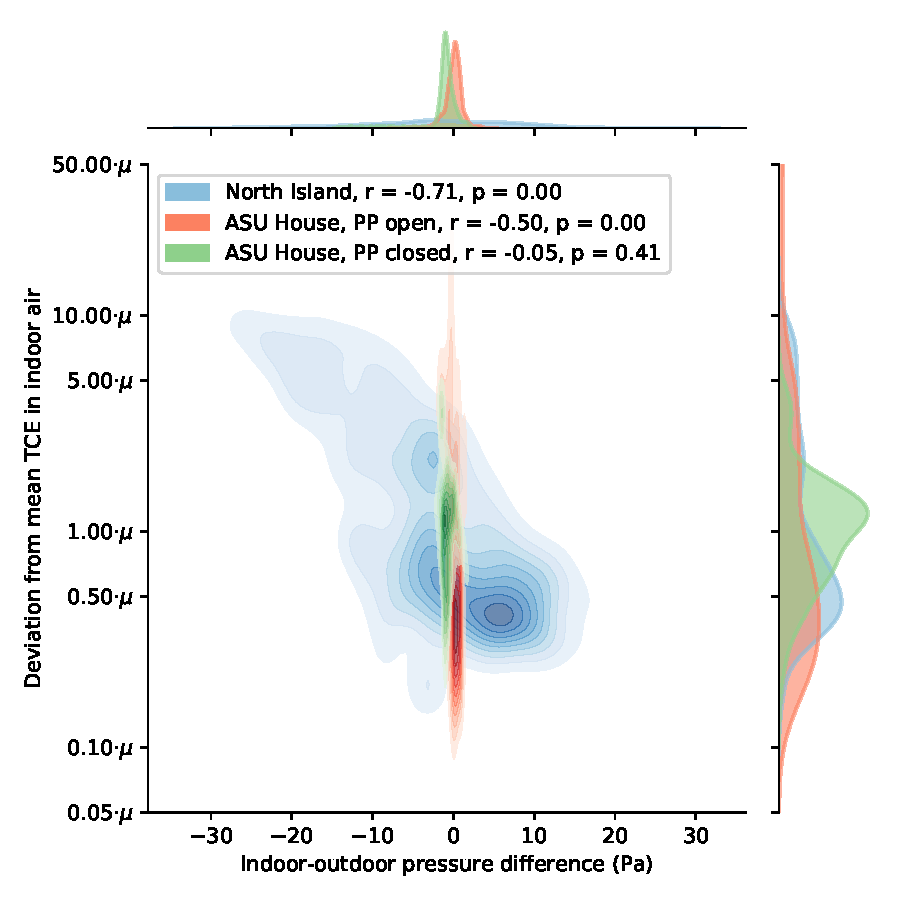
\includegraphics[height=0.4\textheight,keepaspectratio]{nas-asu-house-iacc-deviating.pdf}
  \end{subfigure}
  % Indianapolis plot
  \begin{subfigure}{\textwidth}
    \centering
    \caption{Chloroform and PCE considered at the Indianapolis duplex 422.}
    \label{fig:kde-indianapolis}
    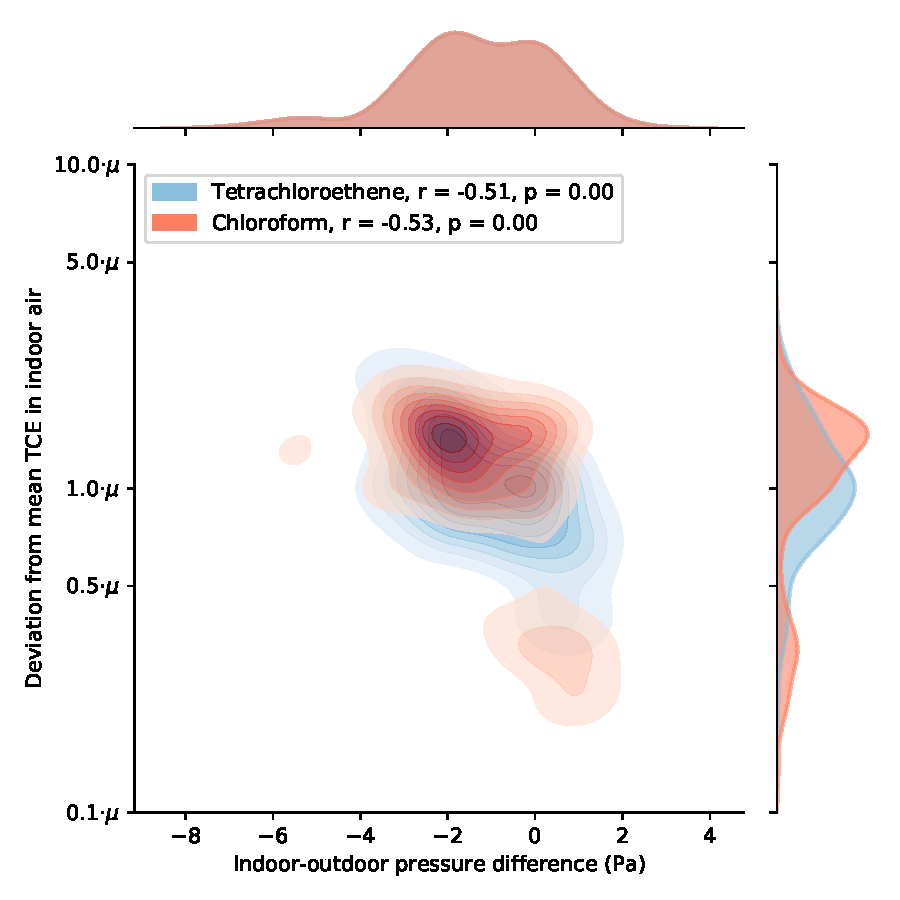
\includegraphics[height=0.4\textheight,keepaspectratio]{indianapolis-422.pdf}
  \end{subfigure}
\end{figure}
% Introduction
Of the factors that influence indoor air contaminant concentration IACC in VI, pressure is one of the most dynamic ones, and the relationship between changes in indoor/outdoor pressure difference and IACC are examined in Figure \ref{fig:kde-analysis}.
Three well-studied VI sites are considered; the "ASU house" near Hill AFB in Utah, a building at North Island NAS in California and a duplex in Indianapolis.\par
% Univariate IACC description
The absolute IACCs at these sites vary significantly, therefore some means of comparing them to each other is necessary.
Additionally, the focus in this section is identifying the driver for variations in IACC, and consistent representation of the variations between the different sites must also be achieved.
Here variations on the scale of orders of magnitude is of interest, as these are of greatest concern in proper site IACC characterization.
To achieve these goals, log-10 deviation from the mean IACC (represented as $\mu$) within each dataset is calculated, e.g. $10\mu$ indicates an IACC that is an order of magnitude above the mean IACC for that dataset.
On the y-margins in Figures \ref{fig:kde-asu-nas} and \ref{fig:kde-indianapolis}, the univariate KDE distribution of deviation from the mean may be seen. \par

What these curves on the y-margins characterize are the distributions of sampled IACC at each site.
Naturally, the distributions are centered around the mean ($\mu = 1$).
In same caes, they look close to simple Gaussians in form (e.g. PCE, Tetrachloroethene at Indianapolis).
In most of the other cases, the distributions are curved and not of a simple nature, strongly suggesting that there might be several factors determinig the IACC. \par

% Univariate pressure description
The indoor/outdoor pressure differences are simply shown as reported, and their univariate KDE distributions are shown on the x-margins.
A negative pressure difference indicates that the building is underpressurized relative to ambient.\par
% Bivariate description
The relationship between the deviation from mean IACC, and indoor/outdoor pressure difference may be seen in the central portion of each figure, in the form of a bivariate KDE distribution.
The p-value and Pearson's r-value for each bivariate distribution are shown in the legend.\par
% Sub-figure description (details about sites)
In Figure \ref{fig:kde-asu-nas} the North Island and ASU house datasets are plotted, with blue representing the North Island site, and with red and green representing the ASU house.
The ASU house dataset is split into two different parts, the first (red) are data from the time period before the preferential pathway was discovered, the second (green) is from after the preferential pathway was sealed off.
At both the ASU house and North Island sites, TCE was the only contaminant considered.
The IACC of Chloroform and PCE in the 422 part of the Indianapolis duplex were considered in Figure \ref{fig:kde-indianapolis}, since they were particulary tracked.\par
% North Island discussion
From Figure \ref{fig:kde-asu-nas}, it is apparent that the three datasets differ significantly from each other.
The North Island site exhibits the greatest variation in both pressure difference and IACC, in fact, looking at the univariate pressure distribution - it is almost entirely flat and spanning from extremly high and low values.
A likely explation for this is the reportedly poor condition of the structure, rendering it highly susceptible to envivornmental influnces.\par

There is also a significant variation in IACC at the North Island site and this has a relativly strong link to pressure difference ($r = -0.71$), although there is clearly a distinct peak (around $0.5\mu$) that is associated with the smaller negative and positive pressure differences ($~-4 \leq \Delta p \leq 8$).
This demonstrates that at this particular site, the very large IACC variations (an order of magnitude or more) are primarily influenced by the unusually large pressure difference fluctations.
Likely, this relationship is created by the fact that the soil surrounding the structure is sandy and therefore relatively permeable - increasing the influence of pressure differences on inflow of contaminant from the soil.
However, despite this, pressure differences can only partly explain the variations observed at this site.\par
% ASU discussion
The two ASU datasets are not only significantly different from the North Island dataset, but also different from each other.
Considering the dataset before the preferential pathway was discovered (red), one can see that the IACC varies significantly (from $0.05 \mu$ to more than $50 \mu$, albeit the latter only rarely.)
This is more variation than was observed at North Island, and yet the observed distribution of pressure differences is narrow, mostly varying by a few Pa around zero (~$\pm 2$ Pa).
With $r = -0.50$, for this dataset, this suggests that pressure difference is not insignificant but still only a weak predictor for the variations in IACC.\par

The picture changes completely after the preferential pathway was closed off, where a similar distribution of pressure differences were observed, but with a signficant reduction in IACC variance to around $\pm 0.5 \mu$, resembling something of a log-normal distribution.
This clearly shows just how much variance the preferential pathway at this site contributed, and how critical it is to assess whether a preferential pathway is present at a particular site since this may lead to large uncertainties in determining relevant contaminant exposures.
It is also clear that in the absence of a preferential pathway, the pressure difference becomes even less important, with the p- and r-value indicating that pressure differences are insignficant in determining variation in IACC.\par
% Indianapolis discussion
The Indianapolis duplex also featured a preferential pathway, but despite this, there is significantly lower variance in IACC for both Chloroform and PCE\cite{mchugh_evidence_2017}.
The exact reason for this is not known, but considering that the preferential pathway at the Indianapolis site was a sanitary sewer, and at ASU the preferential pathway was a foundation drain system, it is not inconceivable that their dynamics are quite different.
Nevertheless, both PCE and Chloroform are more or less log-normally distributed, with (mostly) less than an order of magnitude variance around the mean, indicating that the varations in IACC are species independent.\par

The pressure difference distributions for the Indianapolis site exhibit some bimodal characteristics, with a larger variation than was observed at the ASU site.
This may explain why the r-values for both PCE and Chloroform, $r=-0.51$ and $r=-0.53$ respectively, are so similar to the ASU site before the preferential pathway there was closed; the larger pressure differences, which occured more often than ASU, increase contaminant entry rates to the extent that a preferential pathway was needed to "achieve" at the ASU site.\par
% Summary discussion
All of these data clearly suggest that there is significant variation in IACC that cannot easily be explained by variations in indoor/outdoor pressure difference - even with a preferential pathway.
It is also clear that a preferential pathway may contribute to unacceptable levels of IACC variations, and screening for preferential pathways should be part of any site investiation.
It may also be prudent, even in the absence of a preferential pathway, to add around a half to one order of magnitude margin of error to early screening measurements of indoor air, e.g. if a single sample is less than an order of magnitude below some target limit, it may be justified to perform subsequent sampling to better assess the relevant exposure.
These data also call the role of advection in VI into question, since "normal" pressure difference ranges are such a poor predictor of IACC variation.
This is the opposite of what one would expect if advection were the dominant transport mechanism for entry of contaminant into a structure, under steady-state conditions.\par

\subsubsection{The Role Of Air Exchange Rate}
% Air exchange rate plots
\begin{figure}[htb!]
  \caption{Comparison between the recorded  and the calculated TCE in indoor air at the ASU house, assuming constant air exchange rate. \ref{fig:asu-iacc-ae-overview} shows the TCE in indoor air across time as well as the exchange rate. \ref{fig:violin-iacc-aet} shows the distribution of these values for three periods.}
  \label{fig:ae-analysis}
  % "Overview" plot
  \begin{subfigure}{\textwidth}
    \caption{ }
    \label{fig:asu-iacc-ae-overview}
    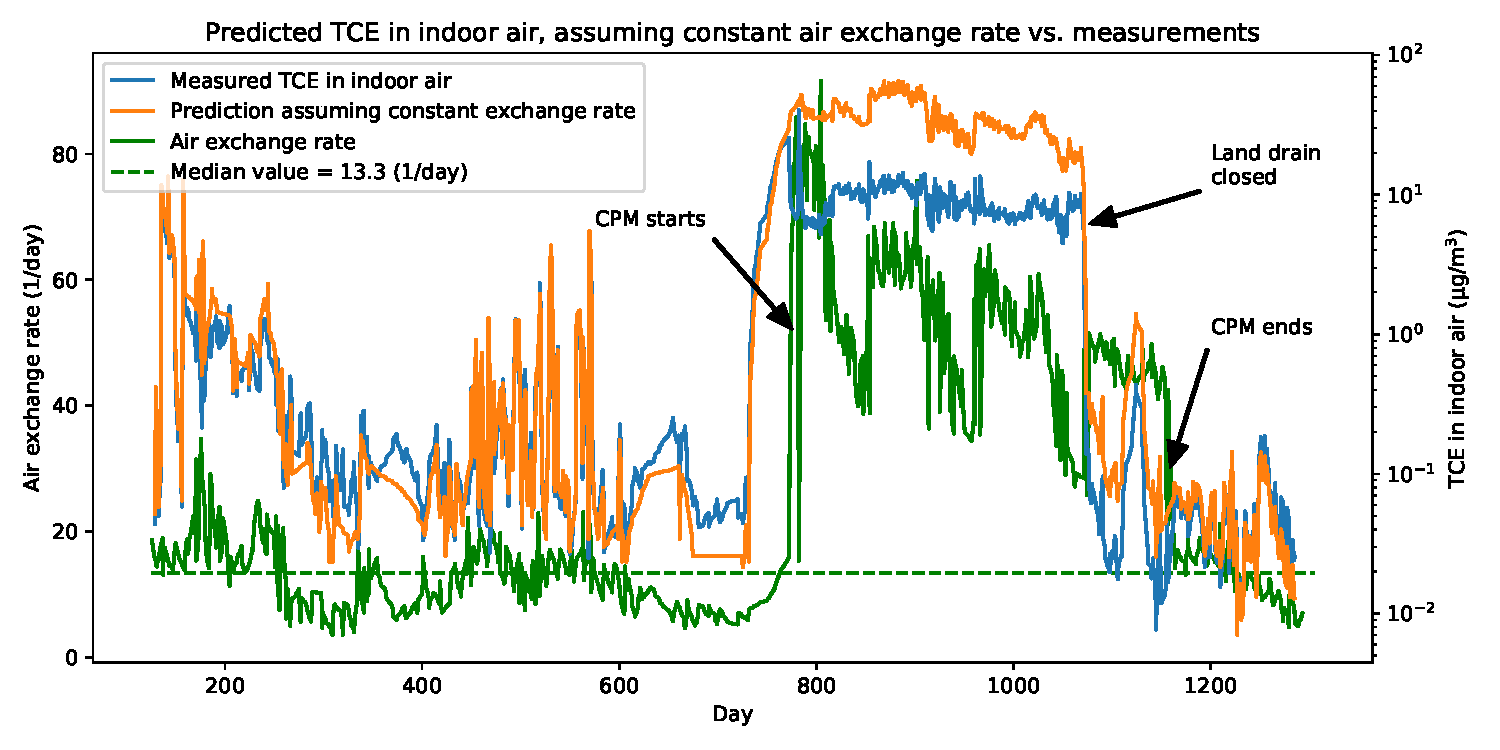
\includegraphics[width=\textwidth]{tce_indoor_air_exchange_rate_impact.pdf}
  \end{subfigure}
  % Violinplot figure
  \begin{subfigure}{0.75\textwidth}
    \caption{ }
    \label{fig:violin-iacc-aet}
    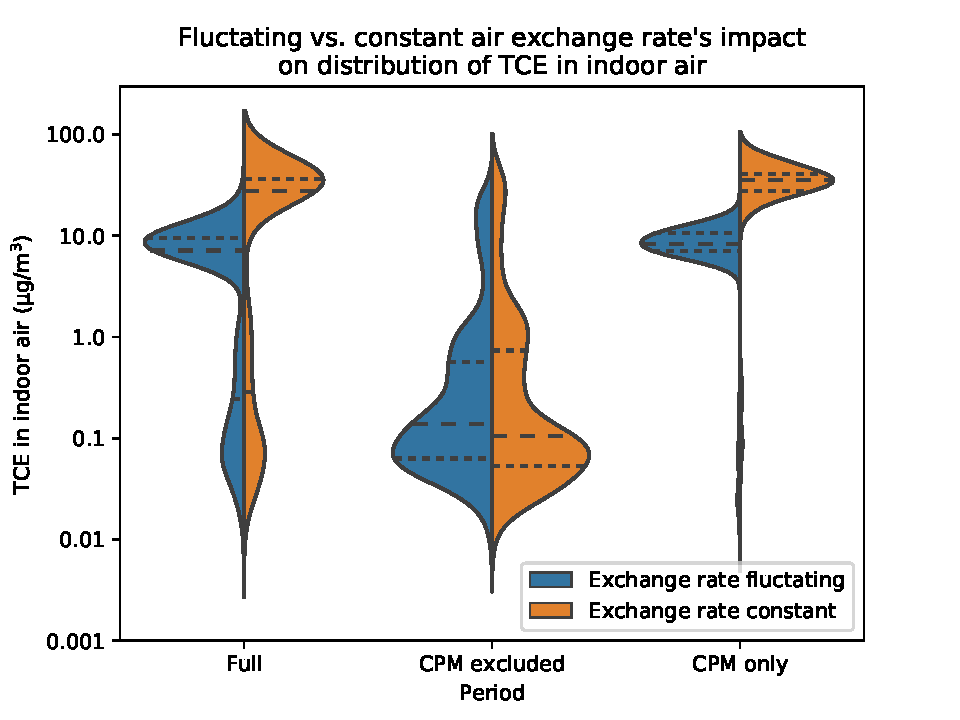
\includegraphics[width=\textwidth]{violin-asu-iacc.pdf}
  \end{subfigure}
\end{figure}
Air exchange rate, which measures how often the interior air in a given building is exchanged with exterior air, is the main parameter characterizing contaminant expulsion, and part of another highly dynamic process.
Exploring the impact of fluctuations in air exchange rate is thus also important for the development of sampling strategies.
At the ASU house, the contaminant entry rate into the structure (called emission rate in that study) as well as the building air exchange rate were recorded across time.
This allows for exploration of the impact that fluctuating air exchange rate has on the final IACC by solving the CST equation, using the recorded contaminant entry rate as one input, and assuming a constant air exchange rate.
The rationale is to show the extent of variability in IACCs due to factors other than fluctuations in air exchange rates.
We have taken this factor out of consideration by below assuming a single constant exchange rate, characteristic of the whole period.

In Figure \ref{fig:asu-iacc-ae-overview}, the measured IACC and air exchange rate across time are shown, compared to the predicted IACC assuming instead a constant air exchange rate.
The median air exchange rate value for the pre-CPM period was chosen as this seemed to be the most representative value for this time period.
From Figure \ref{fig:asu-iacc-ae-overview} it may be seen quite clearly that for the non-CPM periods, the calculated IACC values assuming constant vs. actual fluctuating exchange rates are quite similar.
In other words, in this instance it is unlikely that the variations in IACC were driven by fluctuations in air exchange rate.

This is more clearly shown in Figure \ref{fig:violin-iacc-aet}, where KDEs of the IACC are constructed assuming the constant and fluctuating air exchange rate cases.
This figure shows the relative probability of being at a particular TCE level in indoor air concentration at the ASU house.
These are compared to each other for 1. the full measurement period, 2. the non-CPM periods and 3. the CPM period.
Looking at the full period, it does not appear as though the two cases of steady and fluctuating air exchange rate are comparable, the distribution functions for IACC are different and offset.
The curves to the different sides of the vertical line for the "full" measurement period represent the probability distributions for the indicated values of IACC.
It appears as though assuming a constant air exchange rate shifts the IACC probability distribution to higher values.
The reason for this are more apparent when considering the CPM and non-CPM periods separately.

Considering only the CPM period, assuming a constant air exchange rate does not influence the shape of the IACC distribution, but assuming constant exchange rate shifts the IACC to a higher values.
This is because the actual air exchange rate for this CPM period is significantly higher than the assumed median value, and much more contaminant is actually exchanged with the exterior.
The shape of the IACC distribution is not very different from that which takes the air exchange fluctuations into account, indicating that fluctuating exchange rate is not a major contributor to observed IACC variation for this period (the distinction being drawn between variation and absolute levels of IACC).

The non-CPM period is the condition under which field practitioners would normally collect samples at a VI site.
It is clear here that there is only a very minor difference made in assuming a constant vs. real fluctating air exchange rate, again indicating that accounting for the minor fluctuations of air exchange rate's impact on variations in IACC is not important.
\citeauthor{rackes_time-averaged_2016}\cite{rackes_time-averaged_2016} drew similar conclusions regarding the relationship between IACC and air exchange rate.

\subsection{The Influence of Preferential Pathways}

% Point is:
% If preferential pathways exist, then roughly 1-3 orders of magnitude variability are possible.

% Definition: A preferential pathway is a pathway that allows for contaminant vapor to enter a structure directly or close to the building - circumventing much of the resistance to transport in the soil.

% How do I deal with this? How do I know if preferential pathways may be an issue?

% Scenario: Preferential pathway directly connected to the building.
% - Identify sewer & plumbing fixtures.
% - Drains and sumps may be sources.

% Scenario: Preferential pathway in the near slab area.
% - Permeable sub-base necessary.
% - May have a limited “sphere of influence”.
% -- Limit likely not reached for a normal house.
% -- Limit more likely to be reached for larger structures.

% Relevant for both: Check local manhole/sewer for presence of contaminant - likely source for the preferential pathway.

\subsubsection{Conclusions From Steady-State Modeling}

\begin{figure}[htb!]
  \caption{Sensitivity analysis of IACC dependence on indoor/outdoor pressure difference for cases featuring a preferential pathway (\ref{fig:ss-sensitivity-analysis-pp}) and without a preferential pathway (\ref{fig:ss-sensitivity-analysis-no-pp}). Results compared with field data from ASU house.}
  \label{fig:ss-sensitivity-analysis}
  % "Overview" plot
  \begin{subfigure}{0.45\textwidth}
    \caption{preferential pathway present. Sensitivity to the presence of a gravel sub-base and contamination in the preferential pathway considered.}
    \label{fig:ss-sensitivity-analysis-pp}
    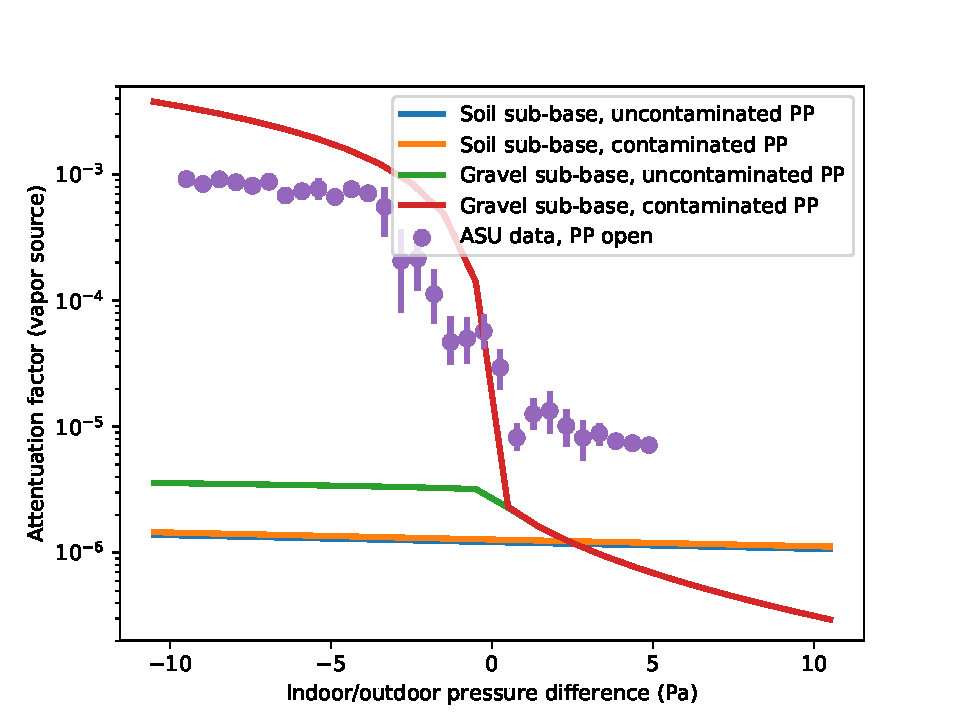
\includegraphics[width=\textwidth]{yes-pp.pdf}
  \end{subfigure}
  % Violinplot figure
  \begin{subfigure}{0.45\textwidth}
    \caption{No preferential pathway present. Sensitivitiy to the presence of a gravel sub-base considered.}
    \label{fig:ss-sensitivity-analysis-no-pp}
    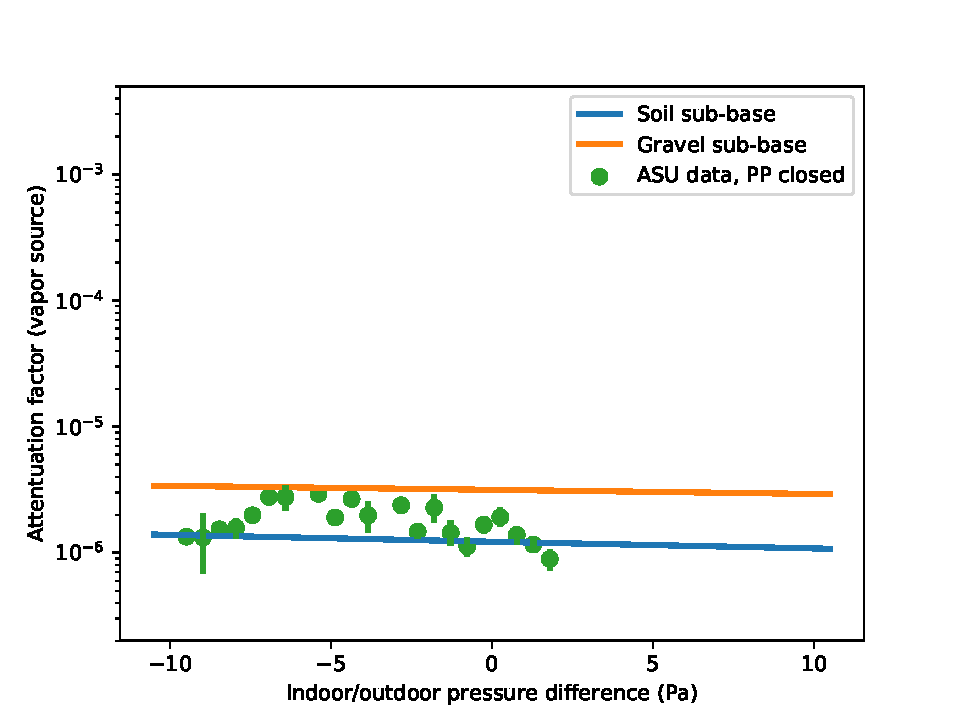
\includegraphics[width=\textwidth]{no-pp.pdf}
  \end{subfigure}
\end{figure}

Clearly, preferential pathways pose a major problem for site investigations, in particular because they may be difficult or even impossible to anticipate or uncover.
Even at a well studied site like the ASU house it took years to discover the preferential pathway.
Therefore, there is a need to consider other indications that a preferential pathway is present or a potential issue.\par

To investigate this, inspiration is taken from the ASU house, where there clearly was a preferential pathway containing contaminant vapor, which exited into a gravel (permeable) sub-base.
The impact of these features is simulated by examining the IACC at different indoor/outdoor pressure differences for each combination of cases.
Instead of representing IACC as absolute concentration, we now non-dimensionalize with respect to the vapor in equilibrium with the groundwater contaminant concentration.
This non-dimensionalized property is commonly called the attenuation factor and is denoted by $\alpha_\mathrm{gw}$.
The result of a steady-state sensitivity analysis relative to several factors is seen in Figure \ref{fig:ss-sensitivity-analysis}.\par

Figure \ref{fig:ss-sensitivity-analysis-pp} deal with cases where a preferential pathway is present and, the impact of having a gravel vs. soil sub-base and vapor contaminant vs. clean air in the preferential pathway ($\chi=1$ and $\chi=0$ respectively) are considered.
Figure \ref{fig:ss-sensitivity-analysis-no-pp} considers the cases absent a preferential pathway, for reference, but still considers the impact of a gravel vs. soil sub-base.
To give perspective to these results, the IACC at the ASU house (as $\alpha_\mathrm{gw}$) vs. indoor/outdoor pressure difference are also plotted.
But the reader is reminded that the model was examined for a structure of the same scale as the ASU house, but which is not an exact representation of it.
Only data from period before the preferential pathway was discovered, and after the preferential pathway was closed are considered in each respective figure (\ref{fig:ss-sensitivity-analysis-pp} and \ref{fig:ss-sensitivity-analysis-no-pp}).
To improve visibility of the ASU data, it's average $\alpha_\mathrm{gw}$ values were aggregated into up to 40 evenly spaced points.\par

Begining with Figure \ref{fig:ss-sensitivity-analysis-pp} it is immediately clear that absent a gravel sub-base, the impact of a preferential pathway is minimal, as comparing the orange and blue lines shows.
Since in the model, it is assumed that the soil type is sandy clay, which is relatively impermeable, there is simply too much resistance to advection in the soil for changes in pressurization to matter.
Additionally, whether the preferential pathway is filled with contaminant vapors or not does not matter; without a permeable sub-base, the transport of contaminant vapor in the sub-base is too slow to allow an advective entry path to contribute with.\par

When a gravel sub-base is present, and the preferential pathway is filled with contaminant vapors ($\chi=1$).
Tthe preferential pathway has a major impact on $\alpha_\mathrm{gw}$, spanning more than four orders of magnitude.
This is explained by the increased role of advective transport under these conditions.
The gravel sub-base allows vapor to readily flow.
When the building is underpressurized under these conditions, a significant amount of contaminant vapor is pulled in from the preferential pathway, leading to the large increase of $\alpha_\mathrm{gw}$.\par

On the other hand, when advection is stopped by overpressurization, most of the contaminant entering the building does so only through diffusion.
This also explains why there is no difference whether the preferential pathway brings only clean air or contaminated air (red and green) when the building is overpressurized.
These two cases differ signficantly from one another when the building is underpressurized, obviously because if there is no additional contaminant being supplied by the preferential pathway, the contaminant comes only from what diffuses from the contaminted groundwater source.\par

It is interesting to note that $\alpha_\mathrm{gw}$ is higher with an uncontaminted preferential pathway (green) entering a gravel sub-base than the cases without a gravel sub-base.
One could expect that pulling so much clean air into the sub-base region might significantly dilute the contaminant vapors and if anything cause a decrease in $\alpha_\mathrm{gw}$ (relative to blue and orange).
However, the preferential pathway is small relative to the dimensions of the sub-base (10 cm diameter pipe), and its impact is only on the contaminant concentration in a limited region of the sub-base.
This gravel sub-base still allows for higher advection throughout the entire sub-base region, leading to a $\alpha_\mathrm{gw}$ plateau that is limited by contaminant transport from the groundwater source, and any small amount of dilution from the preferential pathway is negligible.\par

These case most resembling the ASU site (with an open preferential pathway) is the red case, and the trend agrees with the field data fairly well, especially for small under-/overpressurization values.
The most significant deviations occur as the under-/overpressurization becomes larger.
Again, the model is not intended to replicate the ASU data perfectly, but rather investigate the factors make a preferential pathway the most impactful in a general sense, and perfect simulation is not to be expected.
This is especially reflected in the choice of vapor contaminant concentration in the preferential pathway, with it either being equal to the groundwater contaminant vapor concentration ($\chi=1$) or clean ($\chi=0$), neither of which is likely to be perfectly true at the ASU site.
The idea with picking $\chi=1$ and $\chi=0$ is to give a span of $\alpha_\mathrm{gw}$ values within which a preferential pathway may fall.
This helps explain why $\alpha_\mathrm{gw}$ is overpredicted when the structure is increasingly underpressurized - the contaminant vapor in the preferential pathway at the ASU house was lower than the groundwater contaminant vapor concentration.
The simulation are able to capture the general trends well.\par

In Figure \ref{fig:ss-sensitivity-analysis-no-pp} cases where a preferential pathway is absent are considered, i.e. "normal" VI scenarios, which may be considered reference scenarios.
Here the only issues considered is whether there is a gravel or soil sub-base.
It is apparent that without a preferential pathway, the indoor/outdoor pressure difference changes do not cause any signficant change in $\alpha_\mathrm{gw}$, due to the resistance to advective transport in the surrounding soil - showing the importance of the preferential pathway for increasing advection.
Furthermore, the gravel sub-base does increase the overall $\alpha_\mathrm{gw}$, partly due to slightly higher advective potential but also due to the contaminant vapors being able to more easily diffuse in the more permeable sub-base.
The trend in and even the value sof the data from the ASU house after the preferential pathway had been closed agree well with these model predictions, clearly again demonstrating the role of preferential pathway in increasing advective potential at a site.
It should also be stated that if the surrounding soil was more permeable, e.g. sand, there would be more of a dependence of $\alpha_\mathrm{gw}$ on pressurization, as seen in North Island.\par

Based on the simulated cases in Figure \ref{fig:ss-sensitivity-analysis} it can be concluded that a preferential pathway can be a signficant contributor to VI, but only when particular conditions are met.
\begin{enumerate}
  \item The preferential pathway has to supply additional vapor contaminant.
  \item There must be a source of increased advective potential, which may be due to the presence of the preferential pathway itself, or other site features, or simply due to more permeable surrounding soil.
  \item A permeable sub-base must exist to realize increased advective potential.
\end{enumerate}
In the absense of any of these conditions, a preferential pathway is unlikely to be a signficant contributor to VI.
Strategies for screening for preferential pathway are discussed by \citeauthor{nielsen_remediation_2017}\cite{nielsen_remediation_2017}. \par

\subsubsection{Multivariate Analysis}

\begin{figure}[htb!]
  \caption{Seasonal distribution of relevant VI parameters and indoor air contaminant concentration at the ASU site. Only period after the land drain was closed considered.}
  \label{fig:asu_season}
  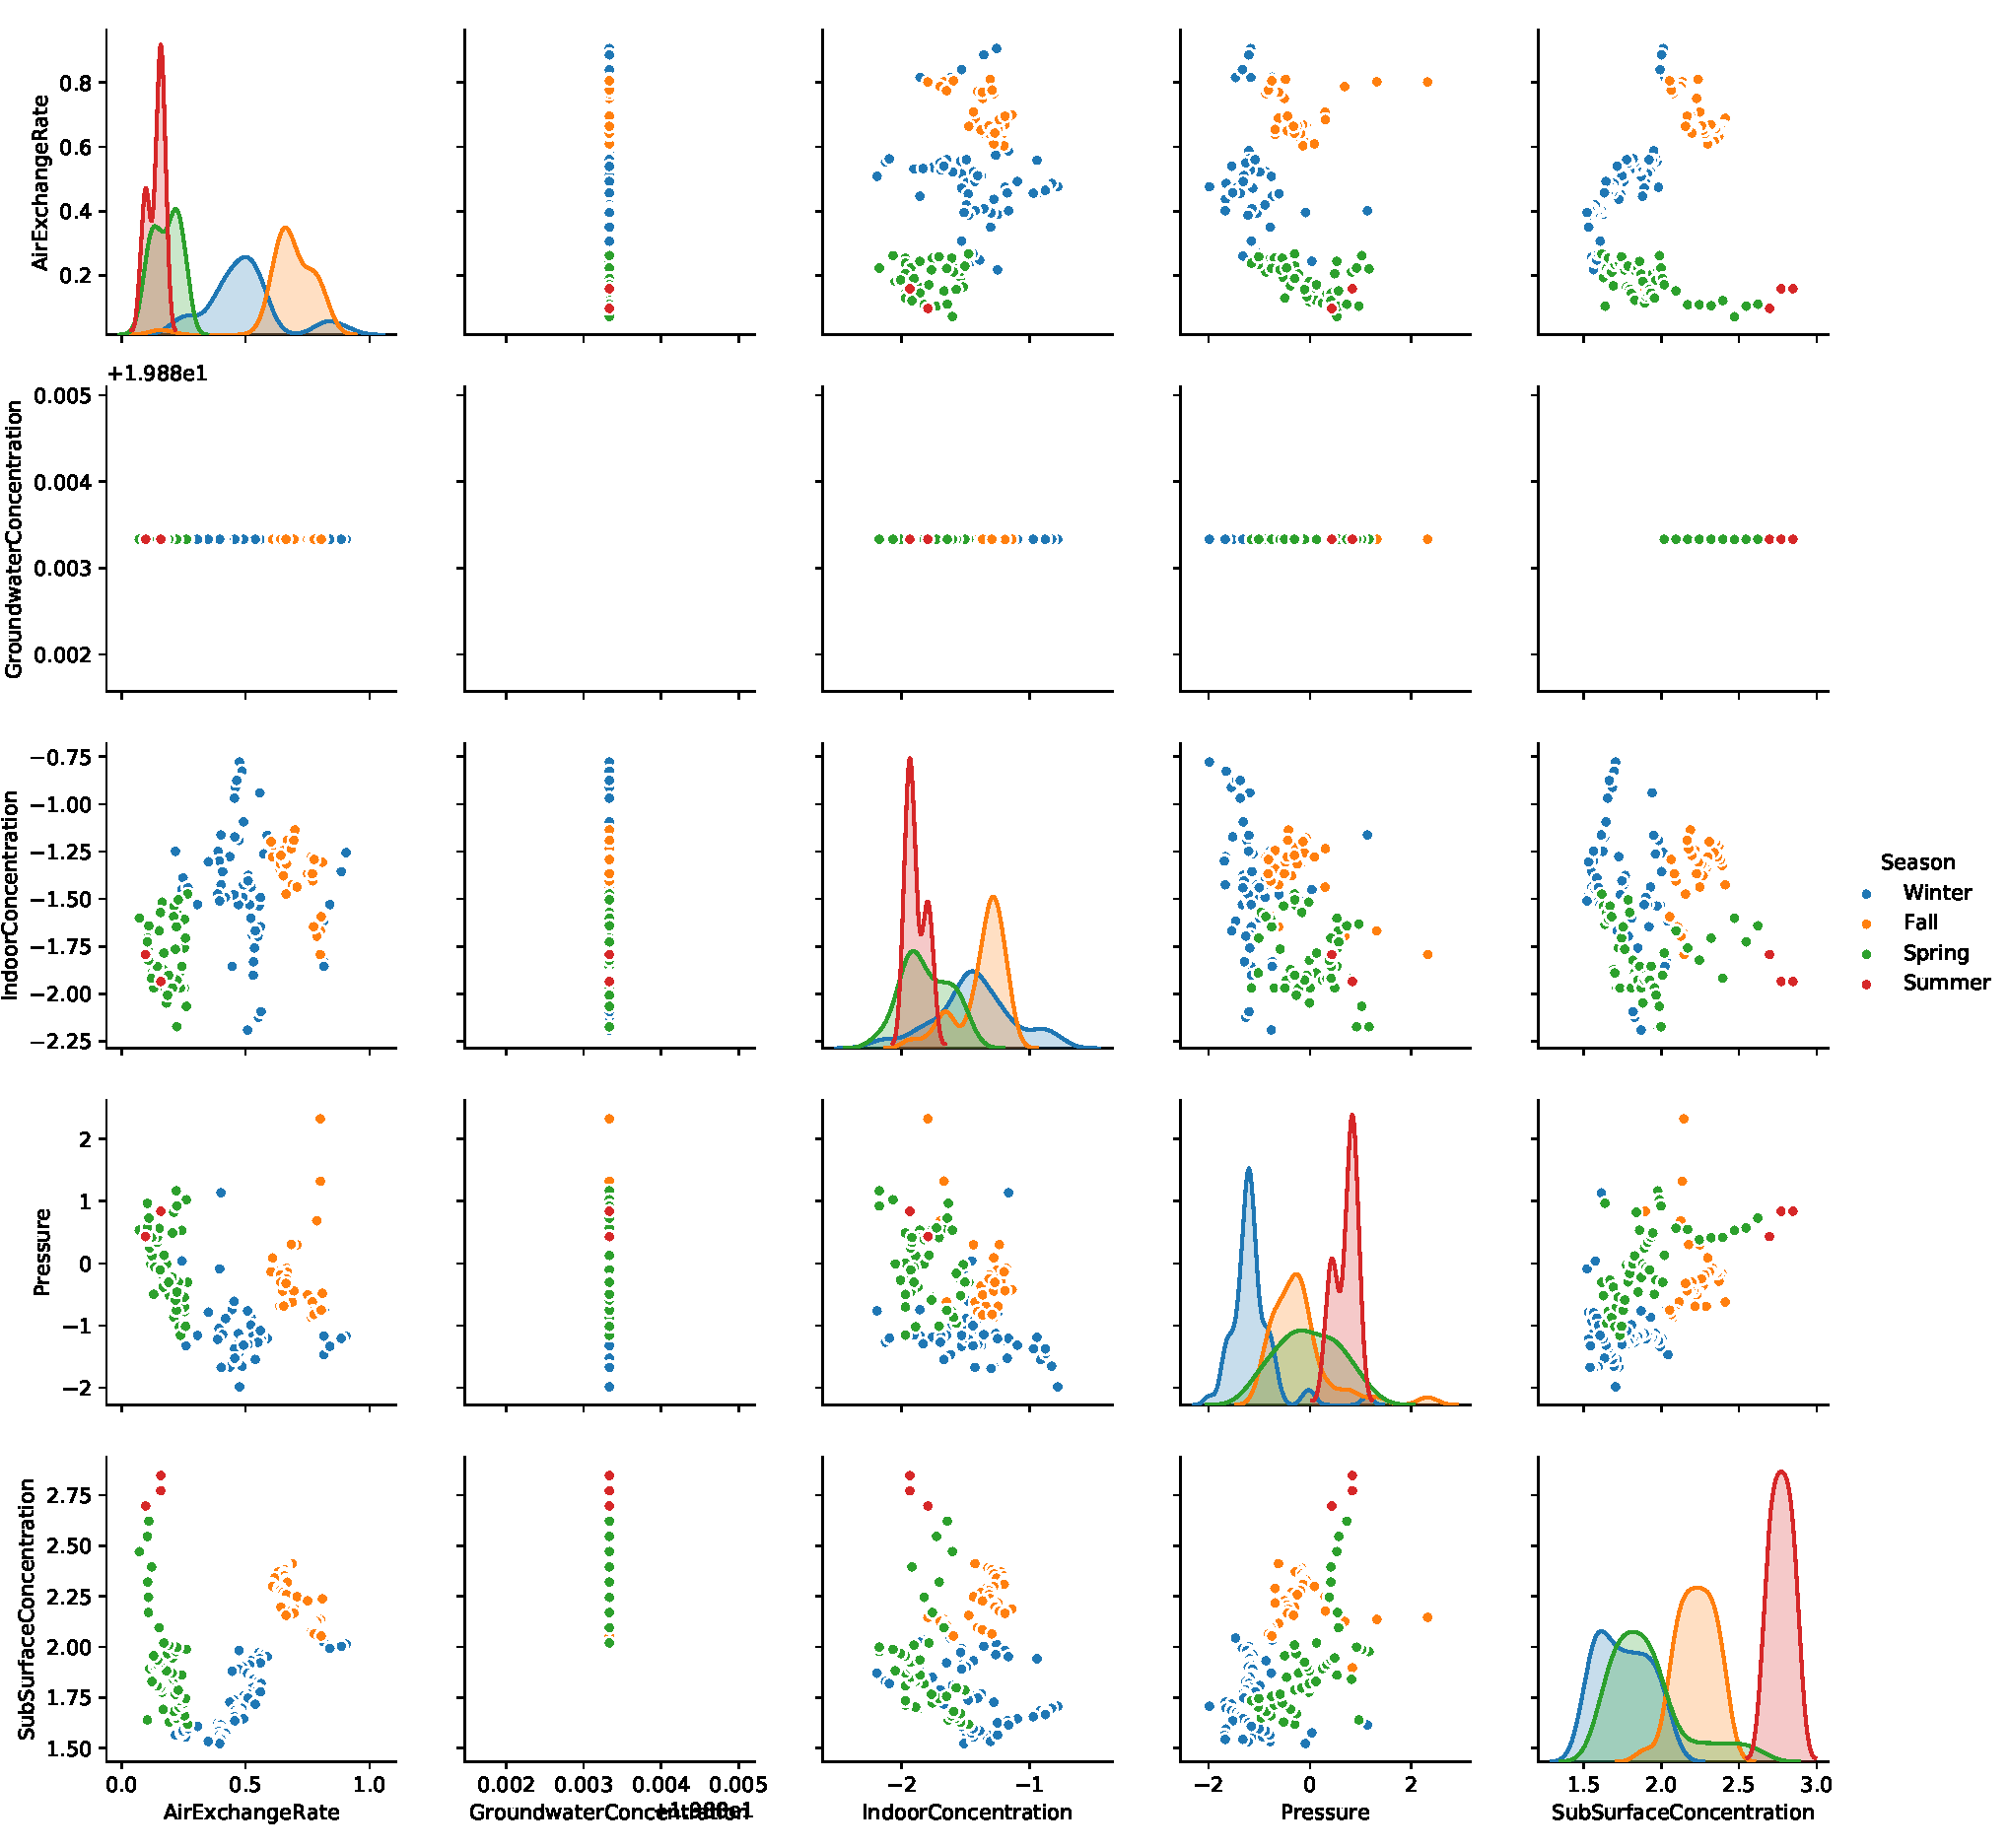
\includegraphics[width=\textwidth]{asu_season.pdf}
\end{figure}

\begin{figure}[htb!]
  \caption{Seasonal distribution of relevant VI parameters and indoor air contaminant concentration at the Indianapolis site. Only PCE considered.}
  \label{fig:indianapolis_season}
  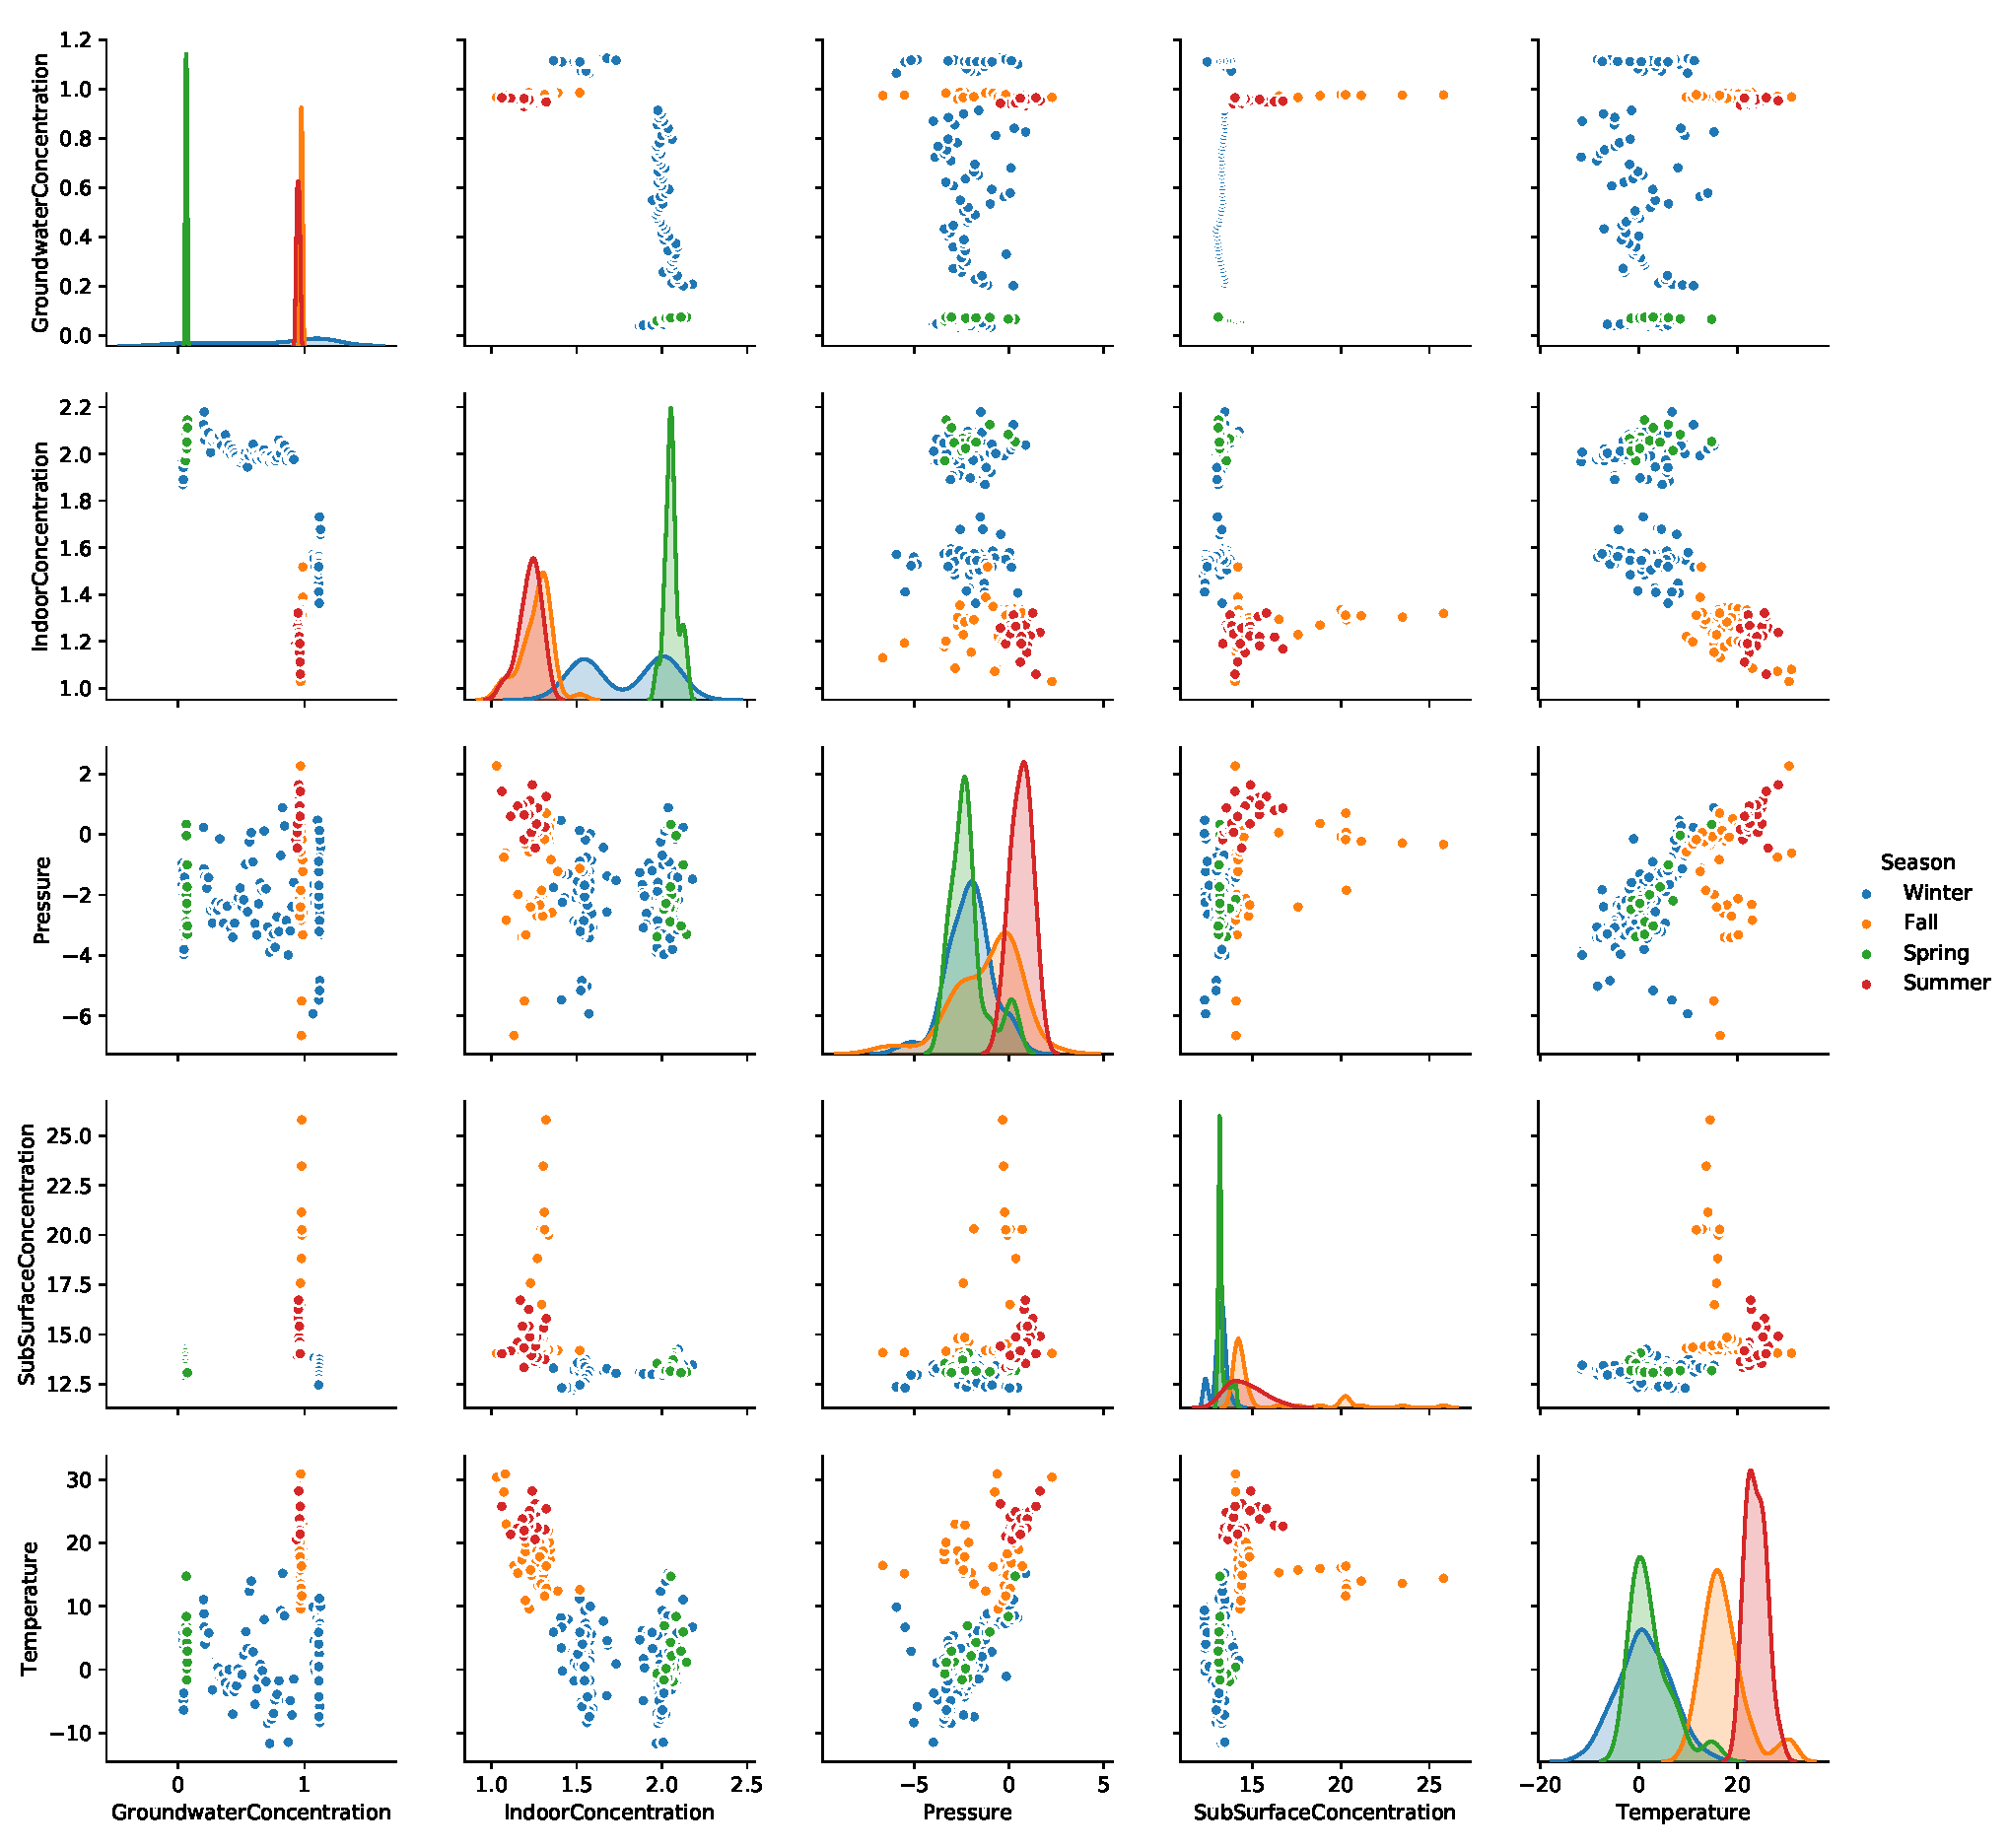
\includegraphics[width=\textwidth]{indianapolis_season.pdf}
\end{figure}

Indoor/outdoor pressure differences or air exchange rate alone do not seem adequately be able to predict the variability observed at the ASU and Indianapolis VI sites, necessitating a multivariate analysis to better understand the distribution of indoor air contaminant concentration.
% TODO: Add references motivating the choice of parameters
This is acheived by examining the distribution various parameters recorded at these sites, and how they relate to eachother.
The distributions of parameters that these two sites share are:
\begin{itemize}
  \item Daily average of the logarithmic indoor air contaminant concentration (TCE at ASU and PCE at Indianapolis).
  \item Daily average groundwater concentration.
  \item Daily average indoor/outdoor pressure difference.
  \item Daily average vapor concentration in the immediate sub-foundation.
\end{itemize}
At the ASU site, the daily average air exchange rate is also given, while at the Indianapolis the daily average outdoor temperature is given.
All of this is shown in Figures (\ref{fig:asu_season}) and (\ref{fig:indianapolis_season}).
It is known that VI potential differs across the seasons, thus the seasonal distribution of each parameter is considered.
Winter is defined as from December to Feburary, spring from March to April, summer from June to August and fall from September to November.
For the ASU site dataset, only the period after the land drain was closed is considered, and the Indianapolis site data only considers the period before the SSD system was installed, and only considers the concentration of PCE.\par

On the diagonal plots in both of these figures, the KDE distributions of each parameter is plotted, with the y-axis denotes the probability density and the x-axis the numeric value associated with that probability density.
The off-diagonals plots are symmetrical, and show the relationship between two parameters.
E.g. in the bottom left plot in Figure \ref{fig:asu_season}, the relationship between the subfoundation TCE concentration and air exchange rate is shown.
A tight cluster resembling a straight line would indicate a linear relationship between the two factors, and the opposite would indicate no real relationship between the two factors exists. \par

What is immediately apparent from these two figures is that there is a very clear seasonal discrepancy between most of the parameters plotted.
Most significant of which is that the indoor air contaminant concentration is the lowest, and exhibit the least amount of variation during summer.
During winter the opposite may be seen, where indoor air contaminant concentations are generally higher, and exhibit higher variabilty.
There is roughly an order of magnitude difference in indoor air concentration between summer and winter, with a few factors (2-3) of variabilty during summer and close to an order of magnitude during winter (albeit this is quite rare).
Indoor air contaminant concentrations fall somewhere inbetween this for the other seasons.
This suggests that maximum VI potential is achieved during winter or colder periods, indicating this may be the best period for VI site investgations, although one should be aware of the larger variability during this period. \par

The reasons for these seasonal trends is not clear by a simple univariate analysis, as has been previously discussed.
This is supported by looking at the relationships between the TCE in indoor air and other parameters in Figure \ref{fig:asu_season}, where no one clear linear relationship exists, but there are some general correlations that can be made, e.g. one can clearly see that higher depressurziation is associated with higher TCE in indoor air.
The TCE in indoor air during summer is a good example of how multiple factors can play a complex role in determining VI potential.
For instance, the subfoundation concentration is the highest during this period, and the air exchange rate is the lowest, which would indicate that the highest concentrations of TCE in indoor air would be found during summer.
But, by looking at the pressure distributions, the house is practically always overpressurized, preventing contaminant entry and reducing variability. \par

At both of these sites, summer is characterized by low contaminant concentrations and low variability as well as a tendency for the structures to be overpressurized, as can be seen in Figure (\ref{fig:indianapolis_season}).
This is likely due to less heating required during warmer periods, removing the stack effect.
It is also interesting to note that at the ASU site, the air exchange rate is the lowest during warmer periods, which is the opposite of what would be expected, as windows and doors are more likely to be open during these periods, increasing air exchange.
However, increasing air exchange rate would simply further decrease indoor air contaminant concentrations during these periods, which is consistent with the previous conclusions.
% TODO: Add reference to the Ae found at different sites during different seasons



\subsubsection{Rates of Change in Indoor Air Contaminant Concentration}

\begin{figure}[htb!]
  \caption{Hourly changes in (logarithmic) indoor air contaminant concentration at the ASU and Indianapolis sites}
  \label{fig:rate_of_change}
  % "Overview" plot
  \begin{subfigure}{0.45\textwidth}
    \caption{ASU site, PP open. Seasonal effect considered.}
    \label{fig:rate_of_change_season_asu_pp_open}
    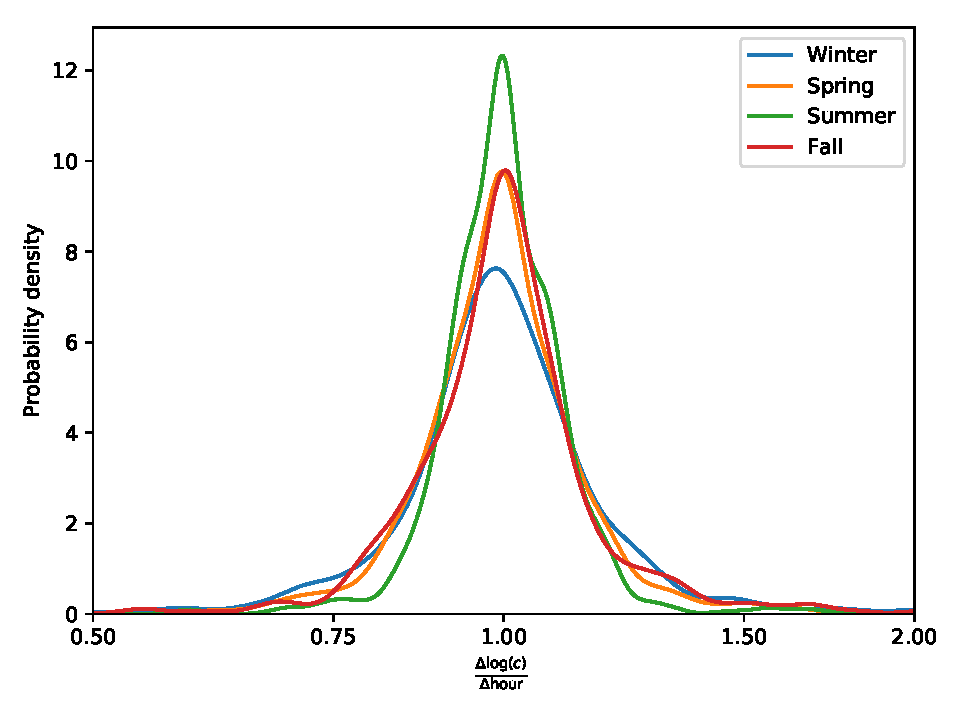
\includegraphics[width=\textwidth]{rate_of_change_season_asu_pp_open.pdf}
  \end{subfigure}
  % Violinplot figure
  \begin{subfigure}{0.45\textwidth}
    \caption{ASU site, PP closed. Seasonal effect considered.}
    \label{fig:rate_of_change_season_asu_pp_closed}
    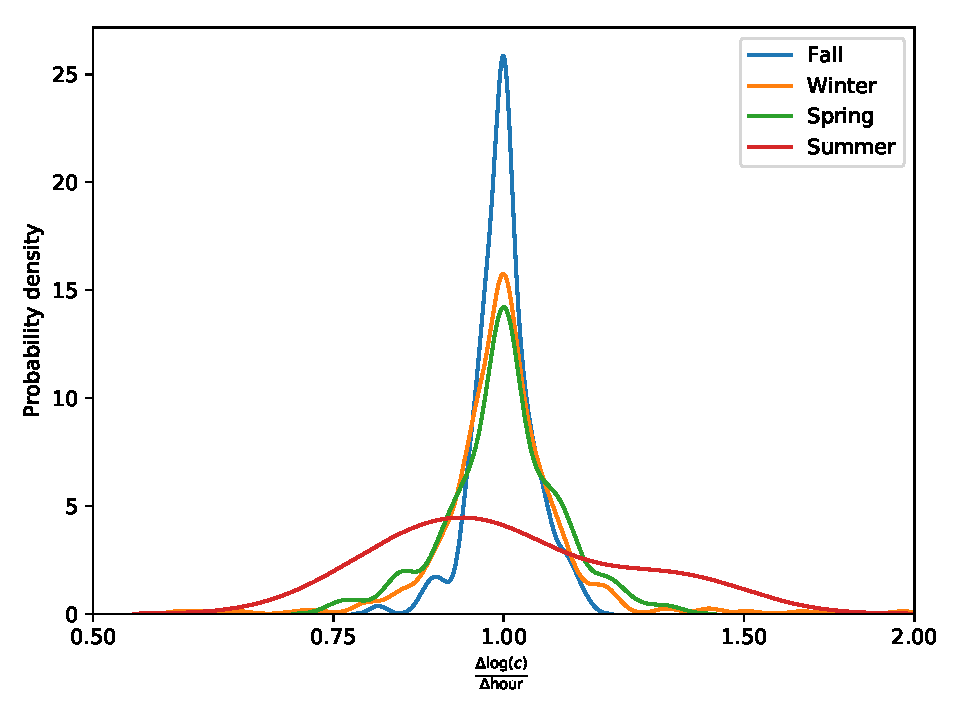
\includegraphics[width=\textwidth]{rate_of_change_season_asu_pp_closed.pdf}
  \end{subfigure}
  % Indianapolis
  \begin{subfigure}{0.45\textwidth}
    \caption{Indianapolis site, only PCE considered. Seasonal effect considered.}
    \label{fig:rate_of_change_season_indianapolis}
    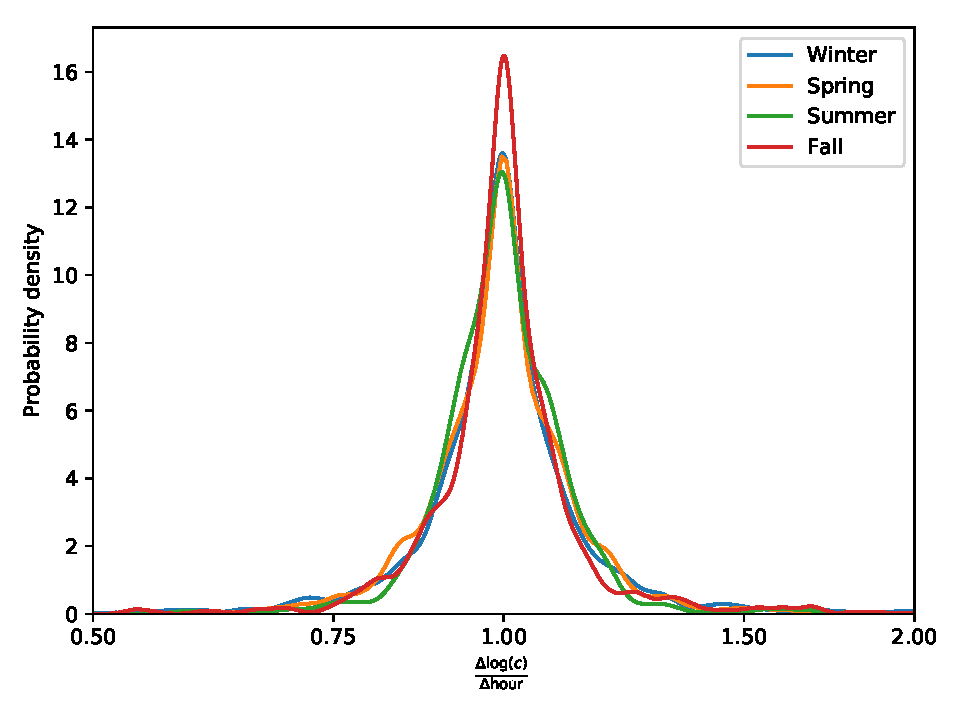
\includegraphics[width=\textwidth]{rate_of_change_season_indianapolis.pdf}
  \end{subfigure}
  % Indianapolis
  \begin{subfigure}{0.45\textwidth}
    \caption{ASU and Indianapolis sites, compared to predicted rates of changes.}
    \label{fig:rate_of_change_simulations}
    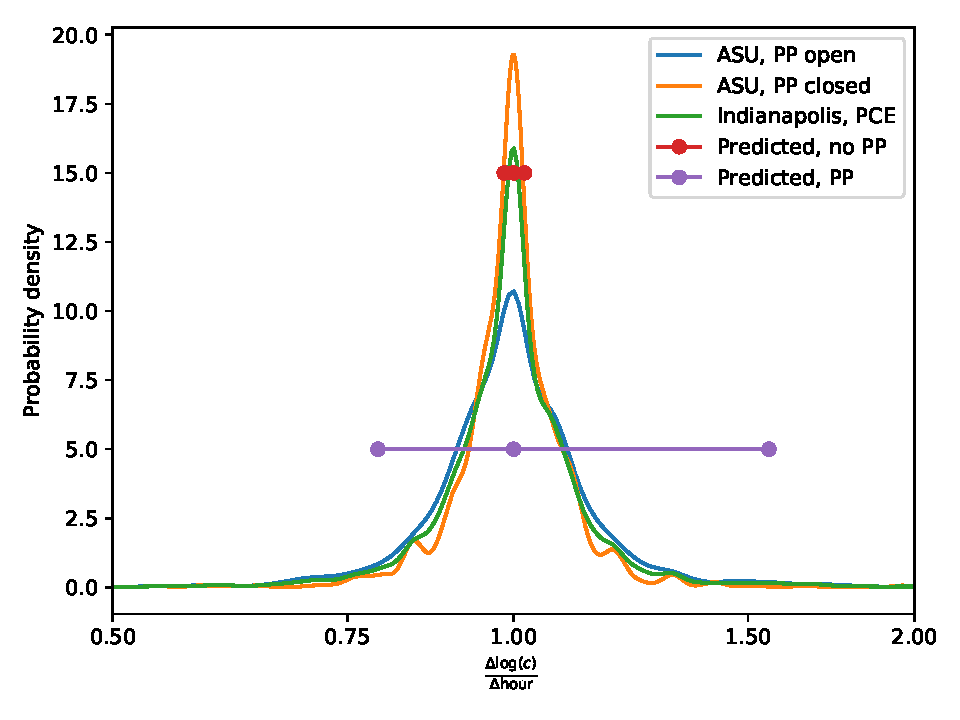
\includegraphics[width=\textwidth]{rate_of_change_simulations.pdf}
  \end{subfigure}
  % "Overview" plot
  \begin{subfigure}{0.45\textwidth}
    \caption{Different resampling frequencies of the Indianapolis site data of the entire ASU site data.}
    \label{fig:resampling_asu}
    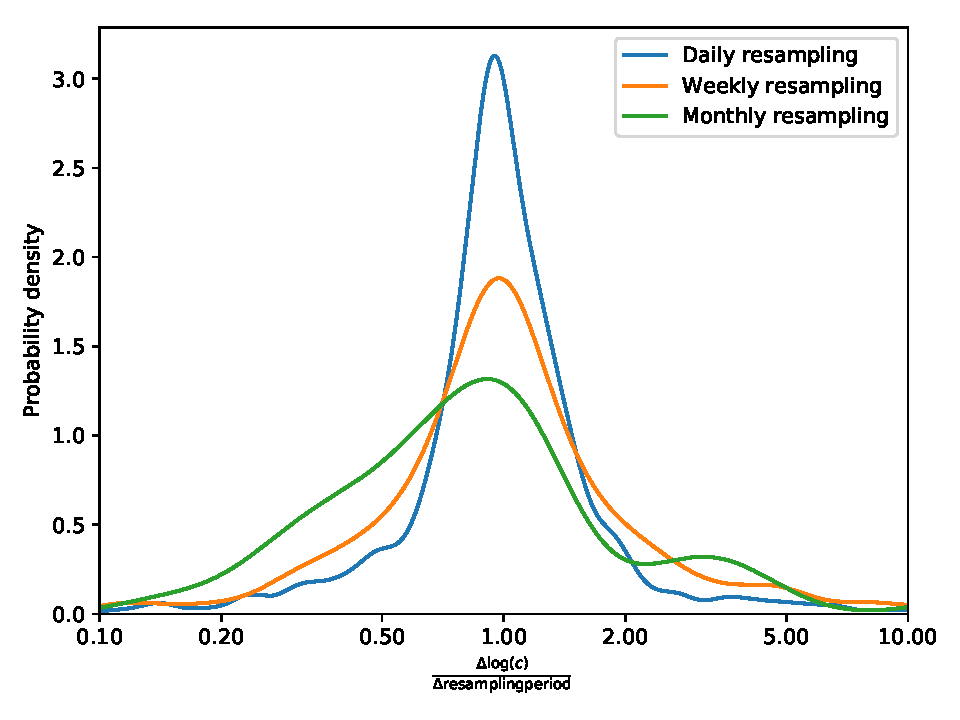
\includegraphics[width=\textwidth]{resampling_asu.pdf}
  \end{subfigure}
  % Violinplot figure
  \begin{subfigure}{0.45\textwidth}
    \caption{Different resampling frequencies of the Indianapolis site data, only PCE considered.}
    \label{fig:resampling_indianapolis}
    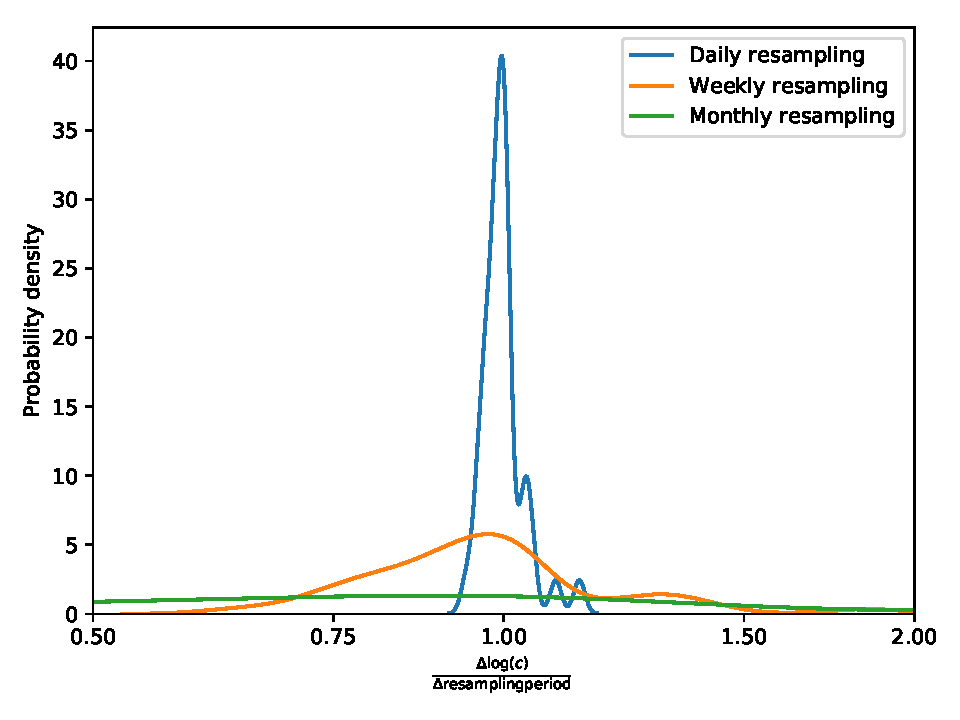
\includegraphics[width=\textwidth]{resampling_indianapolis.pdf}
  \end{subfigure}
\end{figure}

Most of the analysis so far has investigated how various factors impact indoor air contaminant concentrations, but this revleas little regarding how quickly this can change over time.
Knowing how much indoor air contaminant concentration may change over a given time period is important to reduce the number of times indoor air samples have to be collected to establish the relevant indoor air contaminant concentration. \par

To examine this, the ASU and Indianapolis datasets are used again, where the rate of change in indoor air contaminant concentration is calculated, and probability distributions for these valuese given using the KDE method.
The rate of change in indoor air contaminant concentration is given by \eqref{eq:rate_of_change}
\begin{equation}
  \frac{\Delta\log{(c)}}{\Delta t} = \frac{\log{(c(t_2))} - \log{(c(t_1))}}{t_2 - t_1} \label{eq:rate_of_change}
\end{equation}
where $c$ is the indoor air contaminant concentration, $t$ is some timeperiod where the concentration is known and $\log$ is the base-10 logarithm.
In the ASU dataset, indoor air contaminant concentrations were (for the most part) taken at 4-hour intervals\cite{holton_long-term_2015}, while at the Indianapolis site samples were not collected with the same regularity, but several samples were taken everyday for any given sampling location\cite{u.s._environmental_protection_agency_assessment_2015}, giving high time-resolution datasets to work with.

In Figure \ref{fig:rate_of_change_season_asu_pp_open} and \ref{fig:rate_of_change_season_asu_pp_closed} the distributions of the rate of change on an hourly basis, i.e. how much the contaminant concentration changed over one hour ($t_2 - t_1 = 1 \; \mathrm{hour}$), is shown divided up into each season.
Both of the figures consider non-CPM periods, but Figure \ref{fig:rate_of_change_season_asu_pp_open} only contains data from the period when the preferential pathway still open and \ref{fig:rate_of_change_season_asu_pp_closed} data from after the the preferential pathway was closed.

These distributions show that on an hourly basis, only minor changes in indoor air contaminant concentration may be expected; roughly one could at most expect at 50\% increase and a 25\% decrease in indoor air contaminant concentration over a hour at this site.
No significant seasonal difference in the rate of changes seems to exist within either period, except for during summer after the land drain was closed, where greater rates of change indoor air contaminant concentration were more prevalent, albeit still minor.
The preferential pathway had a minor impact on the rate of change, increasing the probability of relatievly greater changes, but again only minor differences.

In Figure \ref{fig:rate_of_change_season_indianapolis} the distribution of hourly rate of change in PCE concentration at the Indianapolis site is shown.
The conclusions from the ASU house hold here as well, with only minor rates of change observed and no seasonal difference.

This suggests that no significant changes in indoor air contaminant concentration may be expected on a hourly basis regardless of the presence of a preferential pathway as well as the hourly rate of change is seasonally independent.

Indoor air contaminant concentrations may however change much more significantly after a longer time period.
This may be investigated by resampling the two datasets over different time periods and aggregating by the mean concentration within each time period.
The rate of change is again calculated using \eqref{eq:rate_of_change}, but unlike in the previous figures, $t_2 - t_1 = 1$ day, week or month.

Since there was no major difference in rate of change in indoor air concentratin between the preferential pathway open/closed periods, the entire non-CPM period of the ASU house dataset is used for this analysis.
Figure \ref{fig:resampling_asu} and \ref{fig:resampling_indianapolis} shows the distributions of rate of change in indoor air contaminant concentration resampled over a daily, weekly and monthly basis at the ASU house and Indianapolis house respectively.

As one might expect, the probability of a larger change in indoor air contaminant increases, as the resampling timeperiod increases.
Only minor changes in indoor air concentration may be expected on a daily basis, albeit larger changes are more likely to occur than on an hourly basis.
At the ASU site, as the resampling timeperiod increases, larger changes become more probable, where on a monthly resampling period half an order magnitude change start to become probable.
At the Indianapolis site, the rate of change over the resampling periods are smaller, and less probable than at the ASU site.
But similarily, after a monthly period, larger changes begin to become more prevalent.

One should keep in mind that by using the mean to aggregate the indoor air concentration, there is a tendency for data to be "smoothed out", missing some of the outliers, especially as the resampling period increases.
Regardless, this analysis suggests that sampling indoor air on a daily basis may be unnecessary as little new information may be gained.
And sampling on a monthly basis may be too long of a period, and important information may be missed.




\begin{acknowledgement}
This project was supported by grant ES-201502 from the Strategic Environmental Research and Development Program and Environmental Security Technology Certification Program (SERDP-ESTCP).
\end{acknowledgement}

\begin{table}[htb!]
  \caption{Abbreviations \& symbols}
  \begin{tabular}{l l}
  \toprule
  \textbf{Abbreviation or symbol}     & \textbf{Explanation} \\
  % General abbreviations
  VI                                  & Vapor intrusion \\
  PP                                  & Preferential pathway \\
  $L_\mathrm{slab}$                   & Thickness of the foundation concrete slab \\
  % Richard's equation
  $p$                                 & Pressure \\
  % Unsteady-cstr
  $u$                                 & TCE in indoor air concentration \\
  $c$                                 & TCE in soil gas concentration \\
  % Diffusion stuff
  $D_\mathrm{air}$                    & Diffusion of TCE in air \\
  $D_\mathrm{water}$                  & Diffusion of TCE in water \\
  $D_\mathrm{eff}$                    & Effective Diffusion of TCE in soil \\
  $K_H$                               & Henry's Law constant \\
  % van Genuchten stuff
  $\theta_g, \theta_w\;\&\;\theta_s$  & Vapor, water filled \& saturated soil porosity \\
  $\theta_r$                          & Residual moisture porosity \\
  $\alpha,\; l,\; n\;\&\; m$          & van Genuchten parameters \\
  $\mathrm{Se}$                       & Soil moisture saturation \\
  $k_r$                               & Relative permeability \\
  $\alpha_\mathrm{gw}$                & Attenuation factor \\
  \bottomrule
  \end{tabular}
\end{table}

\bibliography{library}

\end{document}
